%%%%%%%%%%%%%%%%%%%%%%%%%%%%%%%%%%%%%%%%%
% University/School Laboratory Report
% LaTeX Template
% Used by Haomin Shi @ IIT  for ECE 441
% Created on 8/21/2017
% Version 3.1 (25/3/14)
%
% This template has been downloaded from:
% http://www.LaTeXTemplates.com
%
% Original author:
% Linux and Unix Users Group at Virginia Tech Wiki 
% (https://vtluug.org/wiki/Example_LaTeX_chem_lab_report)
%
% License:
% CC BY-NC-SA 3.0 (http://creativecommons.org/licenses/by-nc-sa/3.0/)
%
%%%%%%%%%%%%%%%%%%%%%%%%%%%%%%%%%%%%%%%%%

%----------------------------------------------------------------------------------------
%	PACKAGES AND DOCUMENT CONFIGURATIONS
%----------------------------------------------------------------------------------------

\documentclass{article}

\usepackage[version=3]{mhchem} % Package for chemical equation typesetting
\usepackage{siunitx} % Provides the \SI{}{} and \si{} command for typesetting SI units
\usepackage{graphicx} % Required for the inclusion of images
\usepackage{natbib} % Required to change bibliography style to APA
\usepackage{amsmath} % Required for some math elements 
\usepackage{enumitem}
\usepackage{textpos}
\usepackage{flafter}
\usepackage[section]{placeins}

\setlength\parindent{0pt} % Removes all indentation from paragraphs

\renewcommand{\labelenumi}{\alph{enumi}.} % Make numbering in the enumerate environment by letter rather than number (e.g. section 6)

%\usepackage{times} % Uncomment to use the Times New Roman font

%----------------------------------------------------------------------------------------
%	DOCUMENT INFORMATION
%----------------------------------------------------------------------------------------

\title{DEPARTMENT OF ELECTRICAL AND COMPUTER ENGINEERING \\ ECE-441 \\ LAB 1} % Title

\author{Haomin \textsc{Shi}} % Author name

\date{\today} % Date for the report

\begin{document}





\maketitle % Insert the title, author and date

\begin{textblock*}{3cm}(14cm, -11cm)
	{via  \LaTeX }
\end{textblock*}



\begin{center}
\begin{tabular}{l r}
Date Performed: & 31/AUG/2017 \\ % Date the experiment was performedalph
Partners: & Anh Nguyen \\ 
Instructor: & Professor Saniie % Instructor/supervisor
\end{tabular}
\end{center}

% If you wish to include an abstract, uncomment the lines below
% \begin{abstract}
% Abstract text
% \end{abstract}

%----------------------------------------------------------------------------------------
%	SECTION 1
%----------------------------------------------------------------------------------------

\section{Introduction}

The main purpose of this lab is for the student to familiarize the equipment, which is the SANPER Educational Lab Unit and the TUTOR software (Courtesy of MOTOROLA\textregistered. This lab will help the student to understand the fundamentals about MC68000 instruction set, especially the functionality of the TRAP \#14 instruction.

\begin{verbatim}MOVE.B #<Function Number>, D7
TRAP #14
\end{verbatim}

% If you have more than one objective, uncomment the below:
%\begin{description}
%\item[First Objective] \hfill \\
%Objective 1 text
%\item[Second Objective] \hfill \\
%Objective 2 text
%\end{description}

\subsection{Background}
\label{background}
\begin{description}
\item[The SANPER ELU:]
The SANPER ELU (Educational Lab Unit) is based on an MC68000 microprocessor made by MOTOROLA\textregistered. The SANPER ELU is developed by Dr. Saniie and Mr. Perich and the unit include multiple peripherals.
\item[MC 68000:]
The MC 68000 is a 16/32-bit CISC microprocessor, which implements a 32-bit instruction set, with 32-bit registers and 32-bit internal data bus, but with a 16-bit main ALU and a 16-bit external data bus, designed and marketed by MOTOROLA\textregistered.
\end{description} 
 
%----------------------------------------------------------------------------------------
%	SECTION 2
%----------------------------------------------------------------------------------------

\section{Lab Equipment and Procedure}
\subsection{Equipment}
\begin{itemize}
\item SANPER ELU
\item TUTOR software
\end{itemize}
\subsection{Procedure}
	\subsubsection{Part A}
		\begin{enumerate}[label=(\alph*)]
		\item Connect SANPER unit
		\item Command testing
			\begin{itemize}
				\item \begin{verbatim}HE <CR>\end{verbatim}  Help Command
				\item \begin{verbatim}DF <CR>\end{verbatim}  Display Formatted Registers Command
				\item \begin{verbatim}.SR 0000 <CR>\end{verbatim}  Modify the value of the Register (e.g: set to zero)
				\item \begin{verbatim}.A1 1234 <CR>\end{verbatim}  Changeing the contents of A1 register to 1234 (\$00001234) or type in the command without the number to examine A1 register
				\item \begin{verbatim}.A <CR>\end{verbatim}  Display all address registers
				\item \begin{verbatim}.D <CR>\end{verbatim}  Display all data registers
			\end{itemize}
		\end{enumerate}
	\subsubsection{Part B}
		\begin{enumerate}[label=(\alph*)]
			\item Assemble program provided (Table 1.1)
			\item Start the program from \$1000
			\item Set the \$900 to output
			\item Run the program
			\item Notice problem
			\item Use trace mode to check register changes
			\item Repeat for programs in Table 1.2 - 1.4
			\item Set SANPER-1 ELU to hardware single-step mode and reset it
			\item Depress the SINGLE STEP PULSE and observe (take pictures)
		\end{enumerate}

%----------------------------------------------------------------------------------------
%	SECTION 3 Result and analysis
%----------------------------------------------------------------------------------------

\section{Result and Analysis}
The result will be showcased in the appendix section B of this lab report. The screenshot of the tutor terminal input will be included in the appendix A section.
	\subsection{Discussion}
		\begin{enumerate}[label=(\arabic*)]
			\item Terminal inputs(program segments) are in the appendix section of this lab report.
			\item Based on the ``mecb\_chapter\_7.pdf'' document, the range of the available memory for user within the SANPER-1 ELU is \$0900 to \$7FFF.
			\item The value of address lines will be listed in the appendix section. For this lab section there is no unusual event. 
			\item Based on the ``mecb\_chapter\_7.pdf'' document, there are two serial ports: 
				%\begin{enumerate}[label=(\arabic*)]
					\begin{tabular}{l r}
						1 - ACIA1: & \$10040 - \$10042 (even) \\
						2 - ACIA2: & \$10041 - \$10043 (odd)\\
					\end{tabular}
				%\end{enumerate}
			\item Based on the ``overview.pdf'' interfaces are:
				\begin{enumerate}[label=(\alph*)]
						\item Parallel Interface/Timer
						\item Peripheral Interface Adapter
						\item Asynchronous Communications Interface Adapter
						\item Serial Port
				\end{enumerate}
			\item ``*AS'', ``*UDS'' and ``*LDS'' means:
				\begin{enumerate}[label=(\alph*)]
					\item ``*AS'' means Address Strobes, it is a three-state signal indicates that the information on the address bus is a valid address.
					\item ``*UDS'' means Upper Data Strobes
					\item ``*LDS'' means Lower Data Strobes
				\end{enumerate}
		\end{enumerate}

%----------------------------------------------------------------------------------------
%	SECTION 4 Conclusions
%----------------------------------------------------------------------------------------

\section{Conclusions}
The lab section is successful. The student was exposed to the SANPER unit and TUTOR program, meanwhile, the student had the chance to put their hands on the system by using The TRAP \#14 call.




%----------------------------------------------------------------------------------------
%	SECTION 5 AA
%----------------------------------------------------------------------------------------

\section{Appendices}
\paragraph{Codes and Terminal Inputs}

	\subsection{Appendix A}
		\subsubsection{Appendix A.1: Original codes with comments}
			\paragraph{\textit{Table 1.1} - Sample Program No.1}
				\begin{verbatim}LEA.L $2000, A7	;load mem
				MOVE.L #$900 ,A5		;set register with address, this line is at $1004
				MOVE.L #$90B ,A6
				MOVE.B #243, D7		;sys call out port 1
				TRAP #14
				MOVE.B #241, D7
				TRAP #14
				MOVE.B #227, D7
				TRAP #14
				BRA $1004	;back to start
				.	;fin
				\end{verbatim}
			\paragraph{\textit{Table 1.2} - Sample Program No.2}
				\begin{verbatim}MOVE.B D0, D1		;d0 to d1 copy, this line is at $900
				MOVE.B #$AA, $1000		;move to a mem address
				BRA $900	;back to start
				.	;end
				\end{verbatim}
			\paragraph{\textit{Table 1.3} - Sample Program No.3}
				\begin{verbatim}MOVE.B D0, D1		;copying, this line is at 900
				MOVE.B #$AA, $1000		;move to a mem address
				BRA $900	;loop back to start
				.	;end
				\end{verbatim}
			\paragraph{\textit{Table 1.4} - Sample Program No.4}
				\begin{verbatim}MOVE.B D0, D1		;copying, @mem $900
				MOVE.B $1000, $1001		;move mem address
				BRA $900	;loop
				.	;end
				\end{verbatim}
			\subsubsection{Actuarial Input}
					\begin{figure}[!htb]
					\begin{center}
					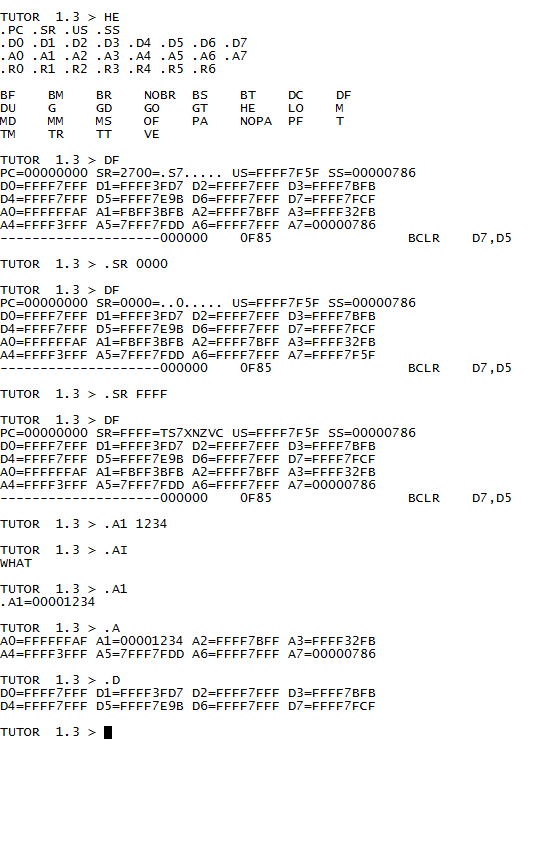
\includegraphics[width=0.65\textwidth]{PARTa} 
					\caption{Part A.1 input}
					%\end{center}
					%\begin{center}
					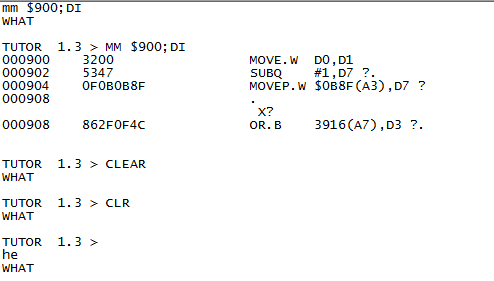
\includegraphics[width=0.65\textwidth]{PARTa1} 
					\caption{Part A.2 input}
					
					\end{center}
			\end{figure}
			%\noindent\rule{8cm}{0.4pt}
					\begin{figure}[!htb]
					\begin{center}
					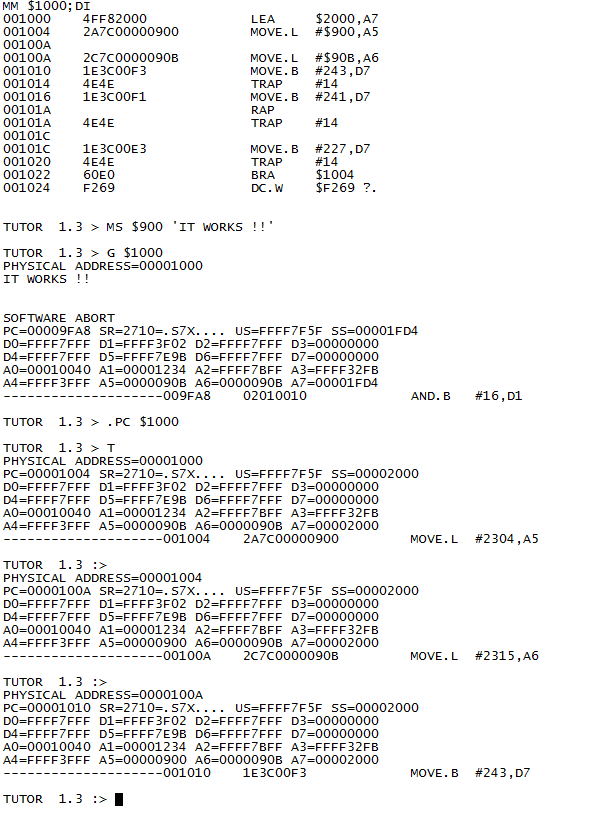
\includegraphics[width=0.65\textwidth]{PARTb} 
					\caption{Part B input}
					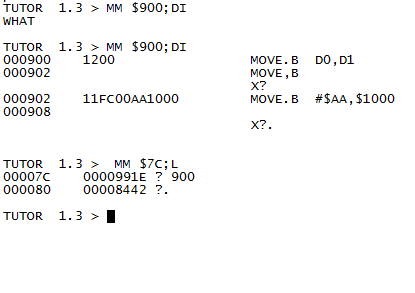
\includegraphics[width=0.65\textwidth]{a} 
					\caption{Part 1.2 input}
					\end{center}\end{figure}
					
					
					\begin{figure}[!htb]
					\begin{center}
					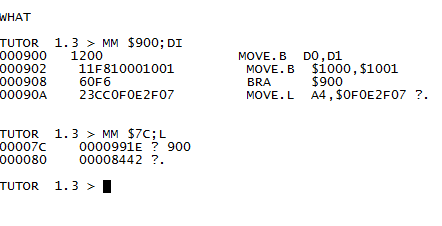
\includegraphics[width=0.65\textwidth]{b} 
					\caption{Part 1.3  input}
					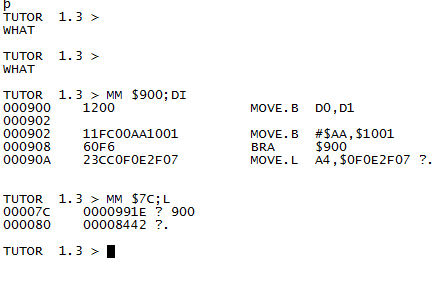
\includegraphics[width=0.65\textwidth]{c} 
					\caption{Part 1.4  input}
					\end{center}\end{figure}
					
\FloatBarrier
			


%----------------------------------------------------------------------------------------
\subsection{Appendix B}
					\begin{figure}[!htb]
					\begin{center}
					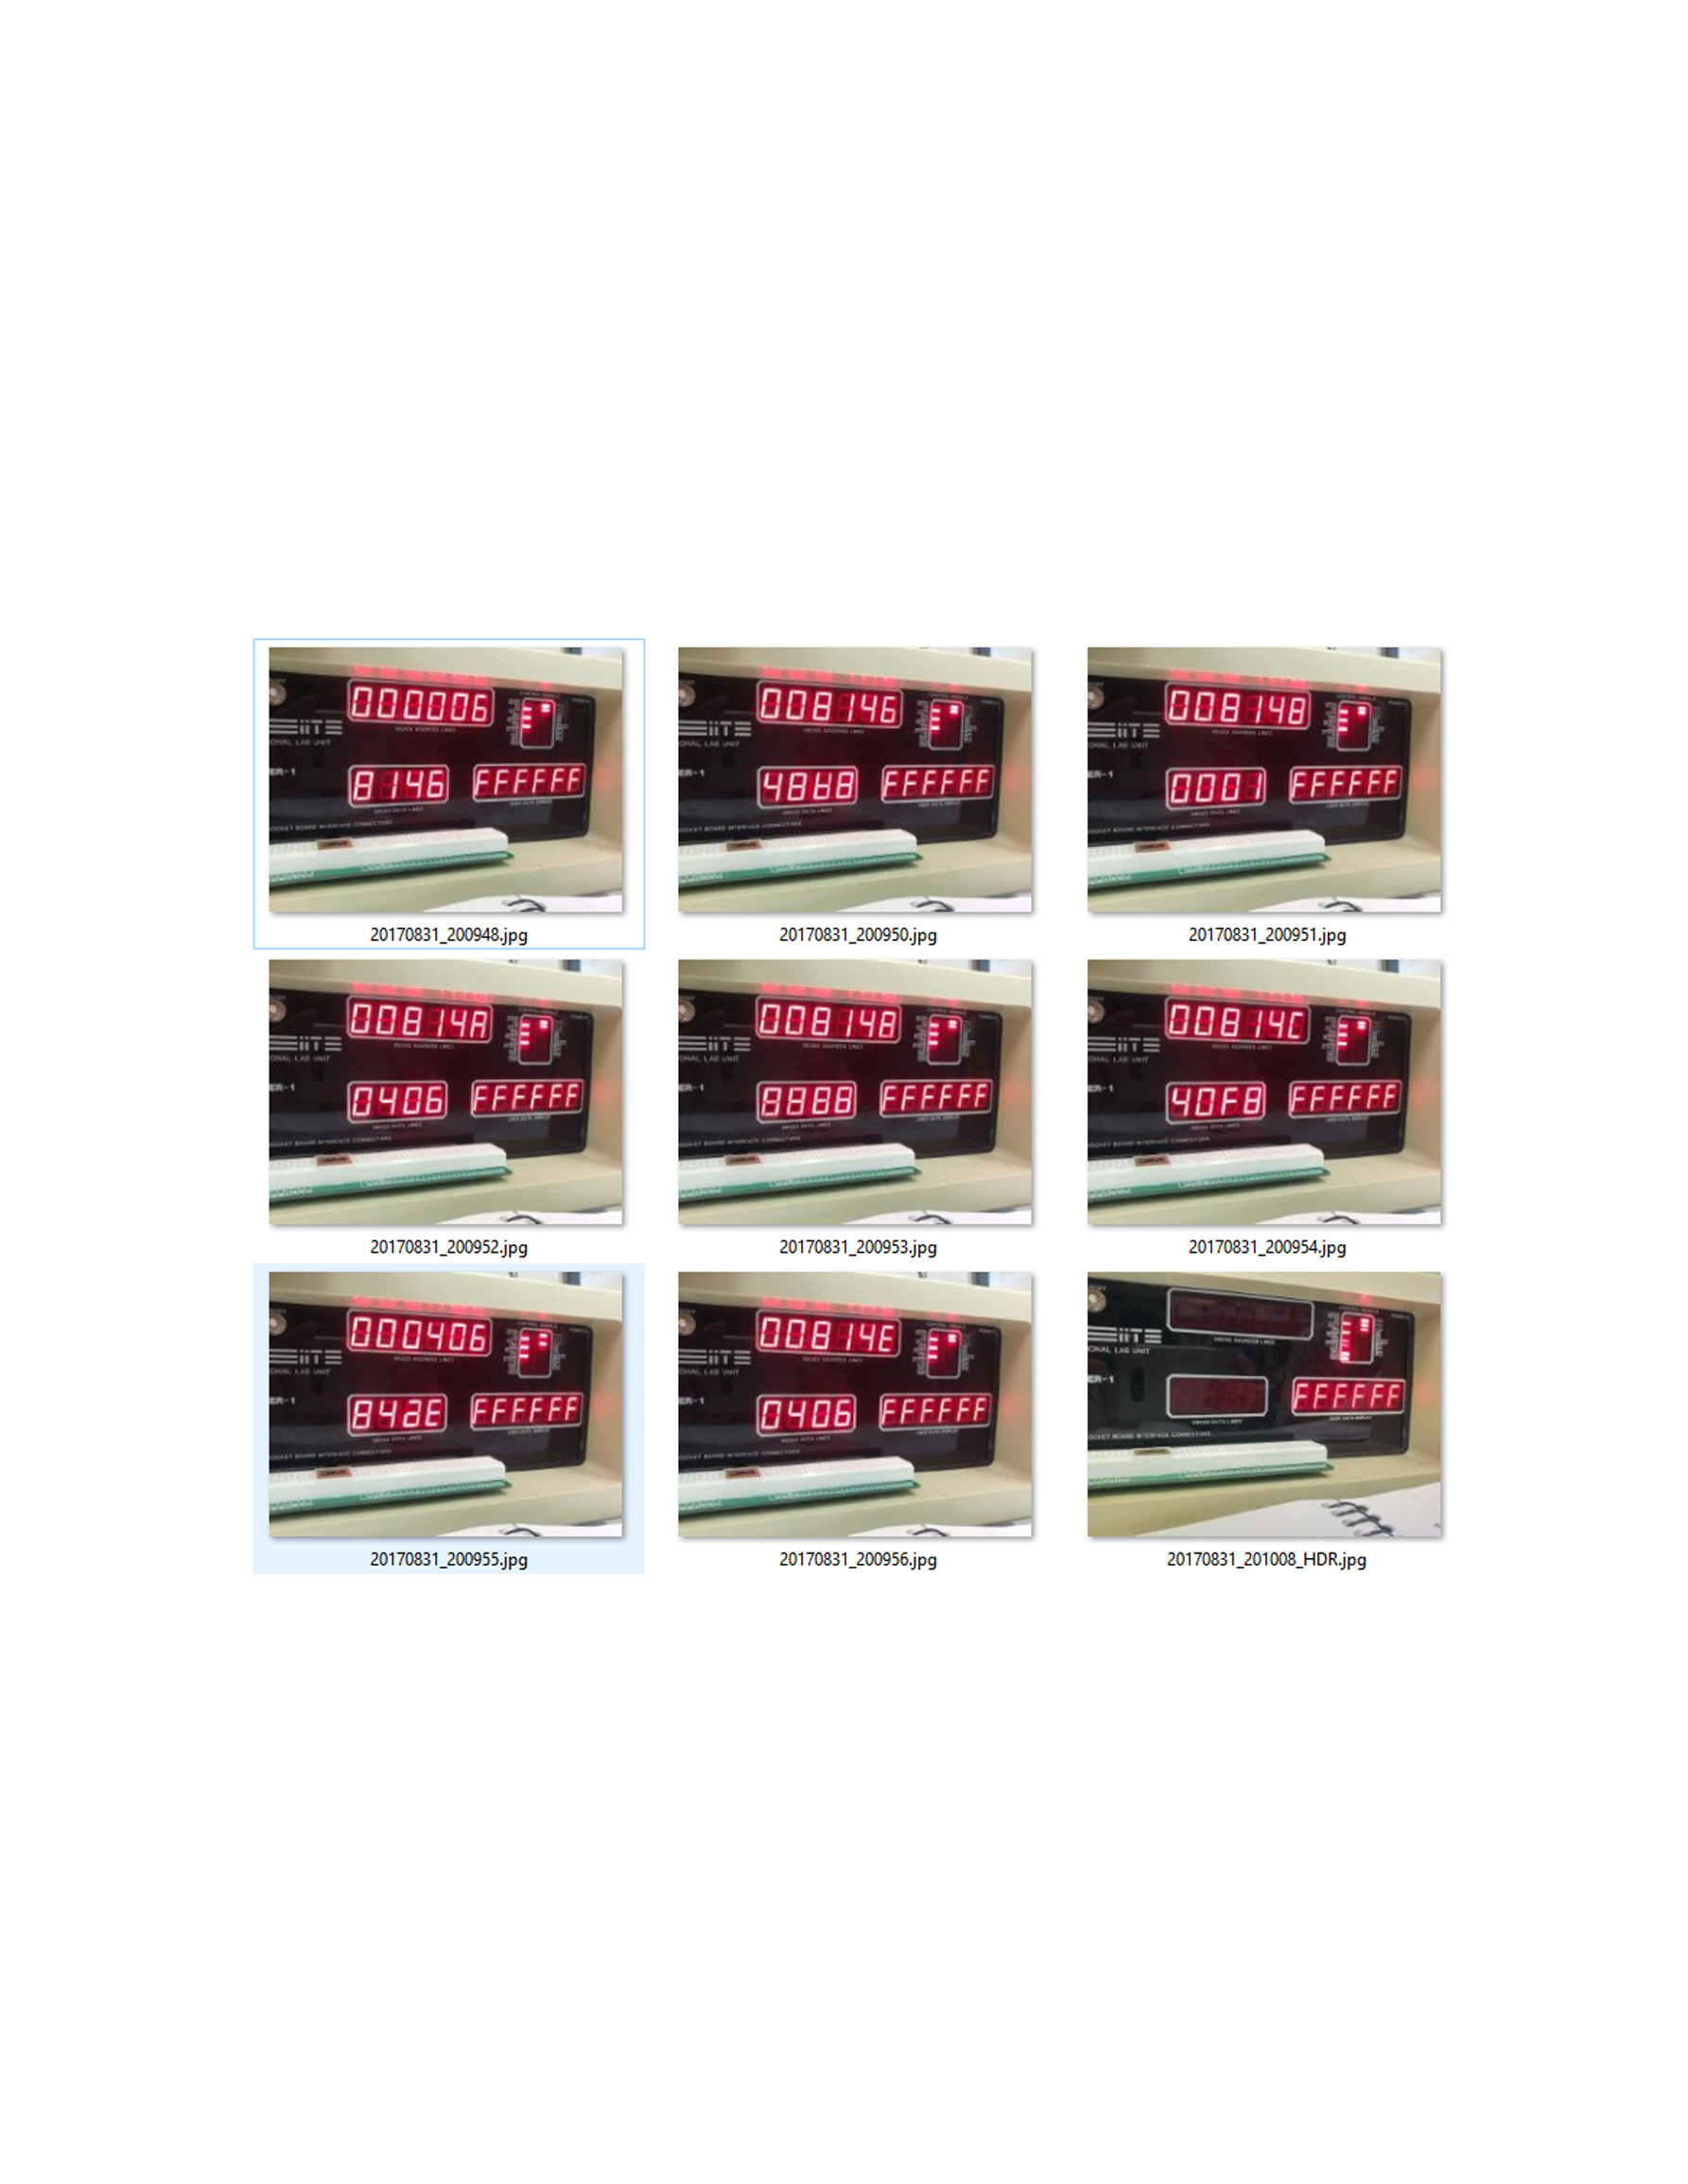
\includegraphics[width=0.9\textwidth]{b5}
					\end{center}\end{figure}
					\begin{figure}[!htb]
					\begin{center}
					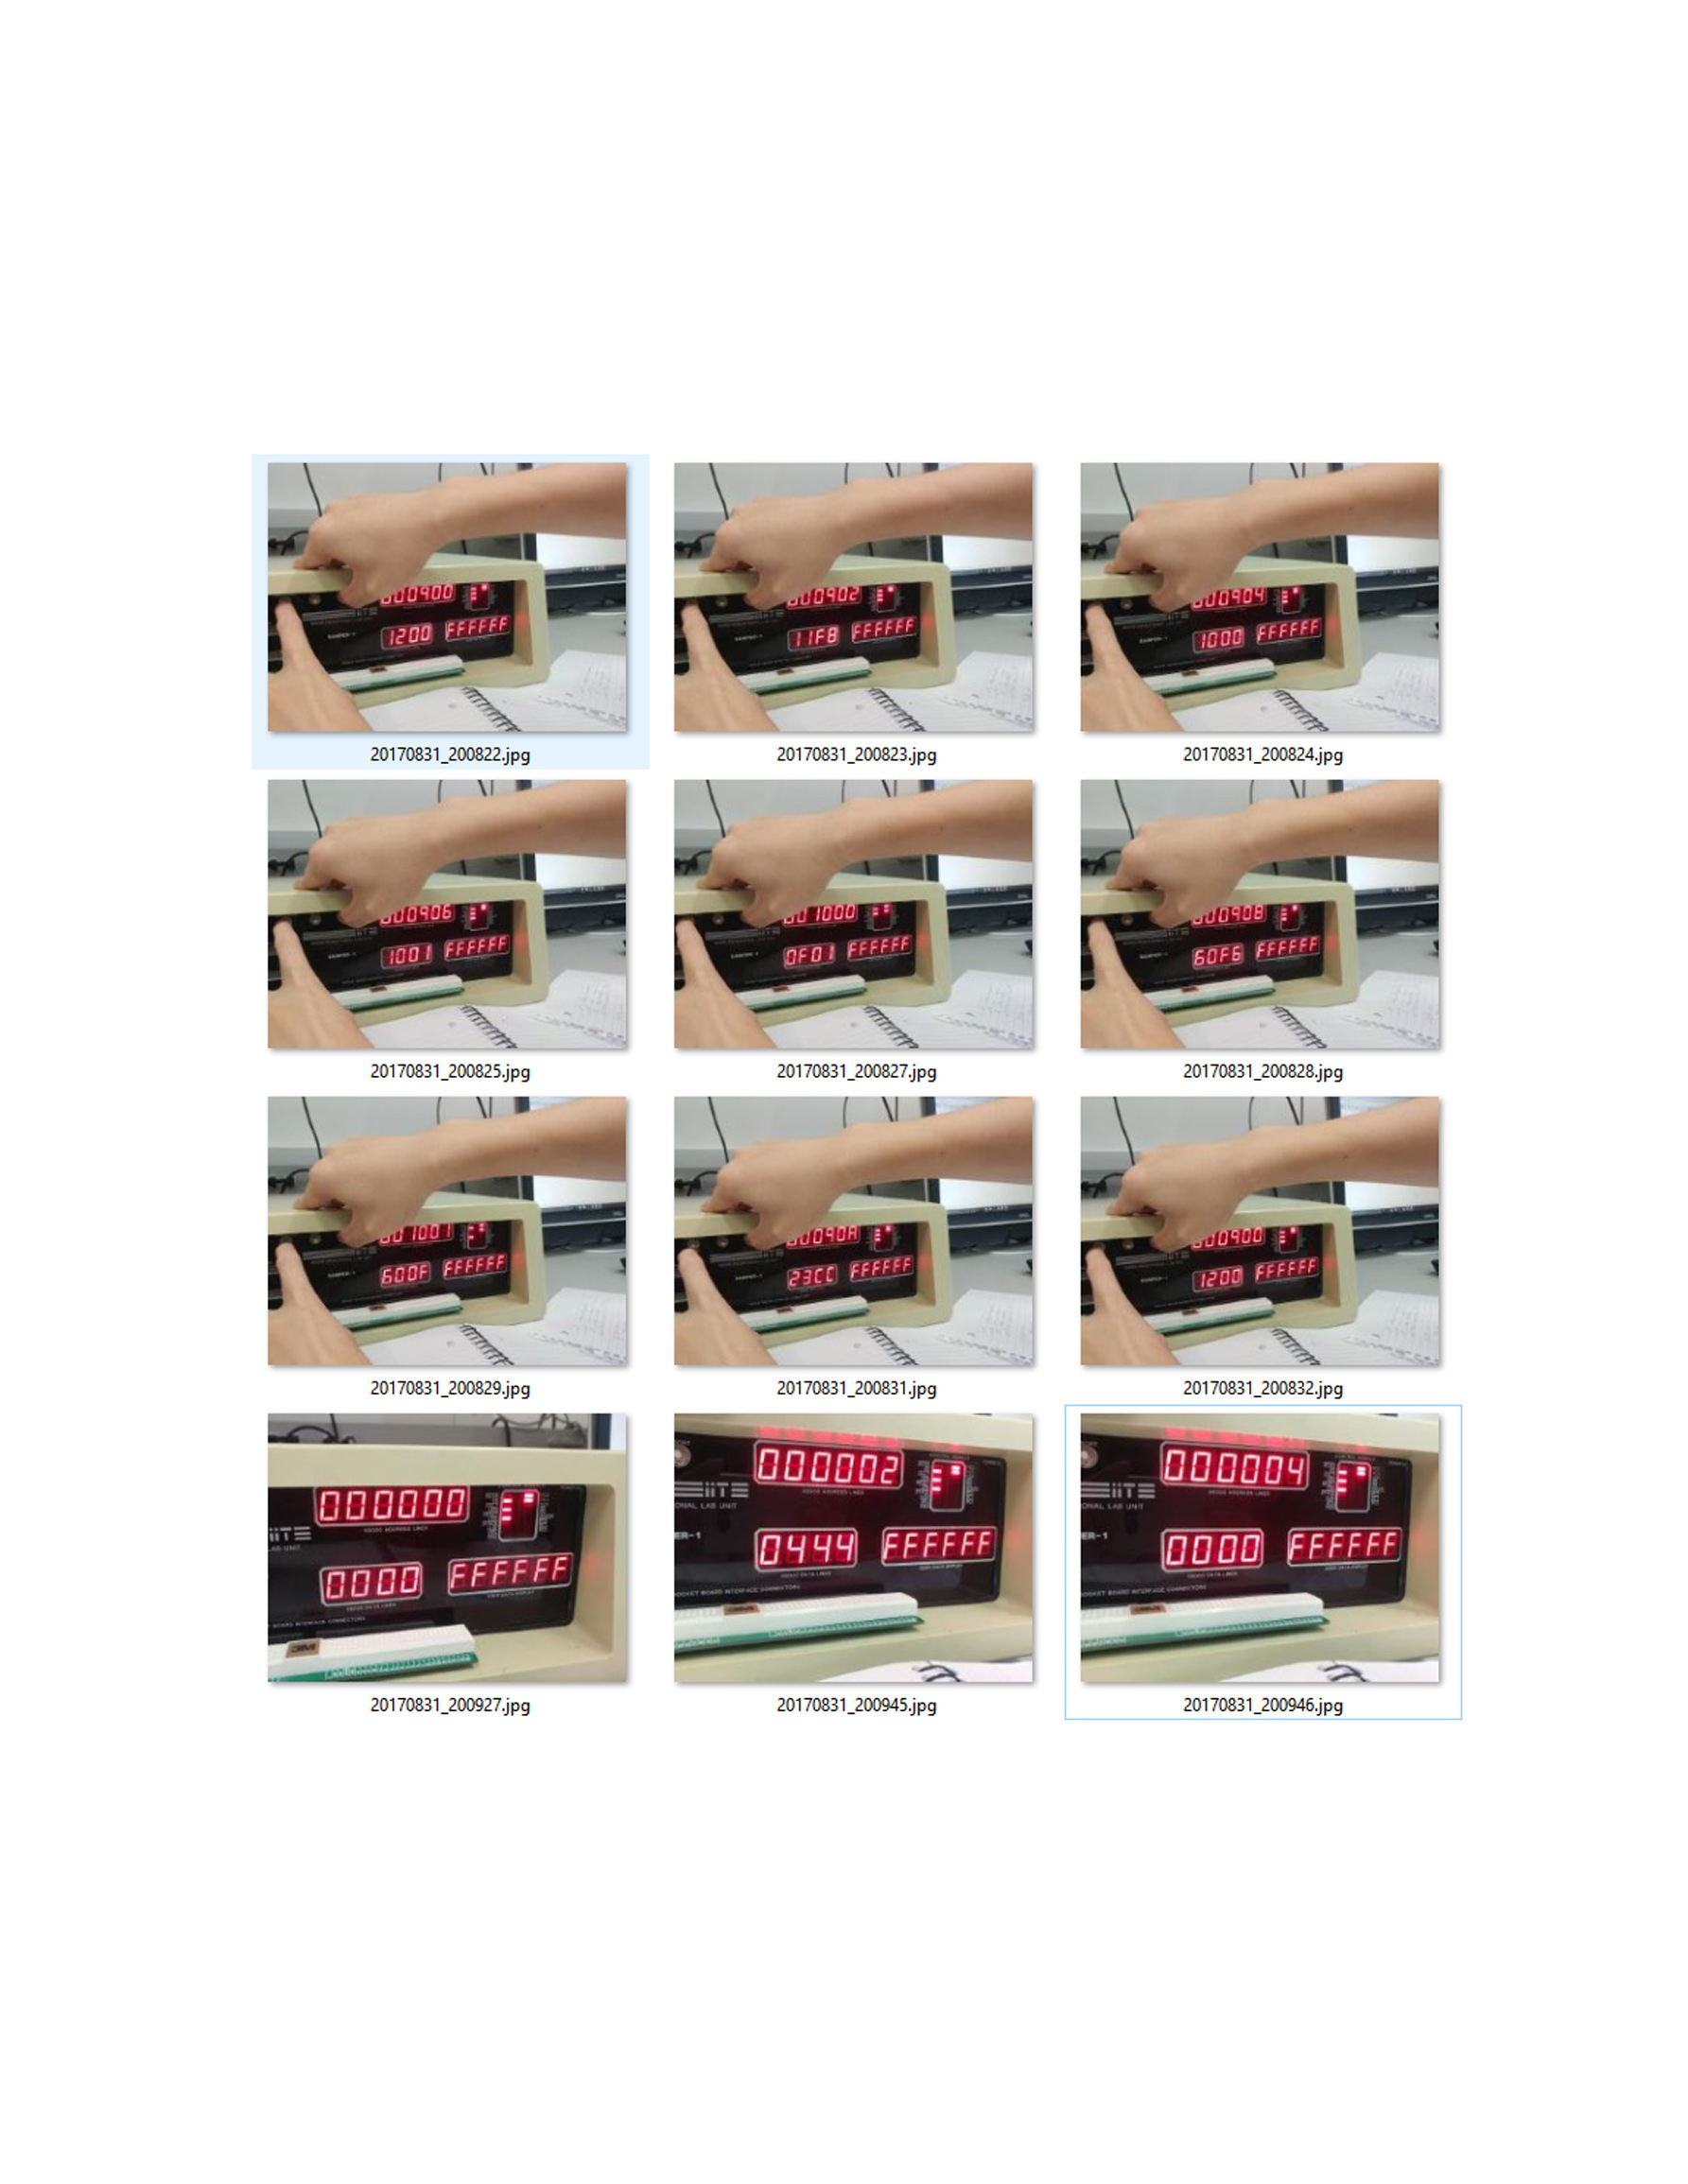
\includegraphics[width=0.9\textwidth]{b4}
					\end{center}\end{figure}
					\begin{figure}[!htb]
					\begin{center}
					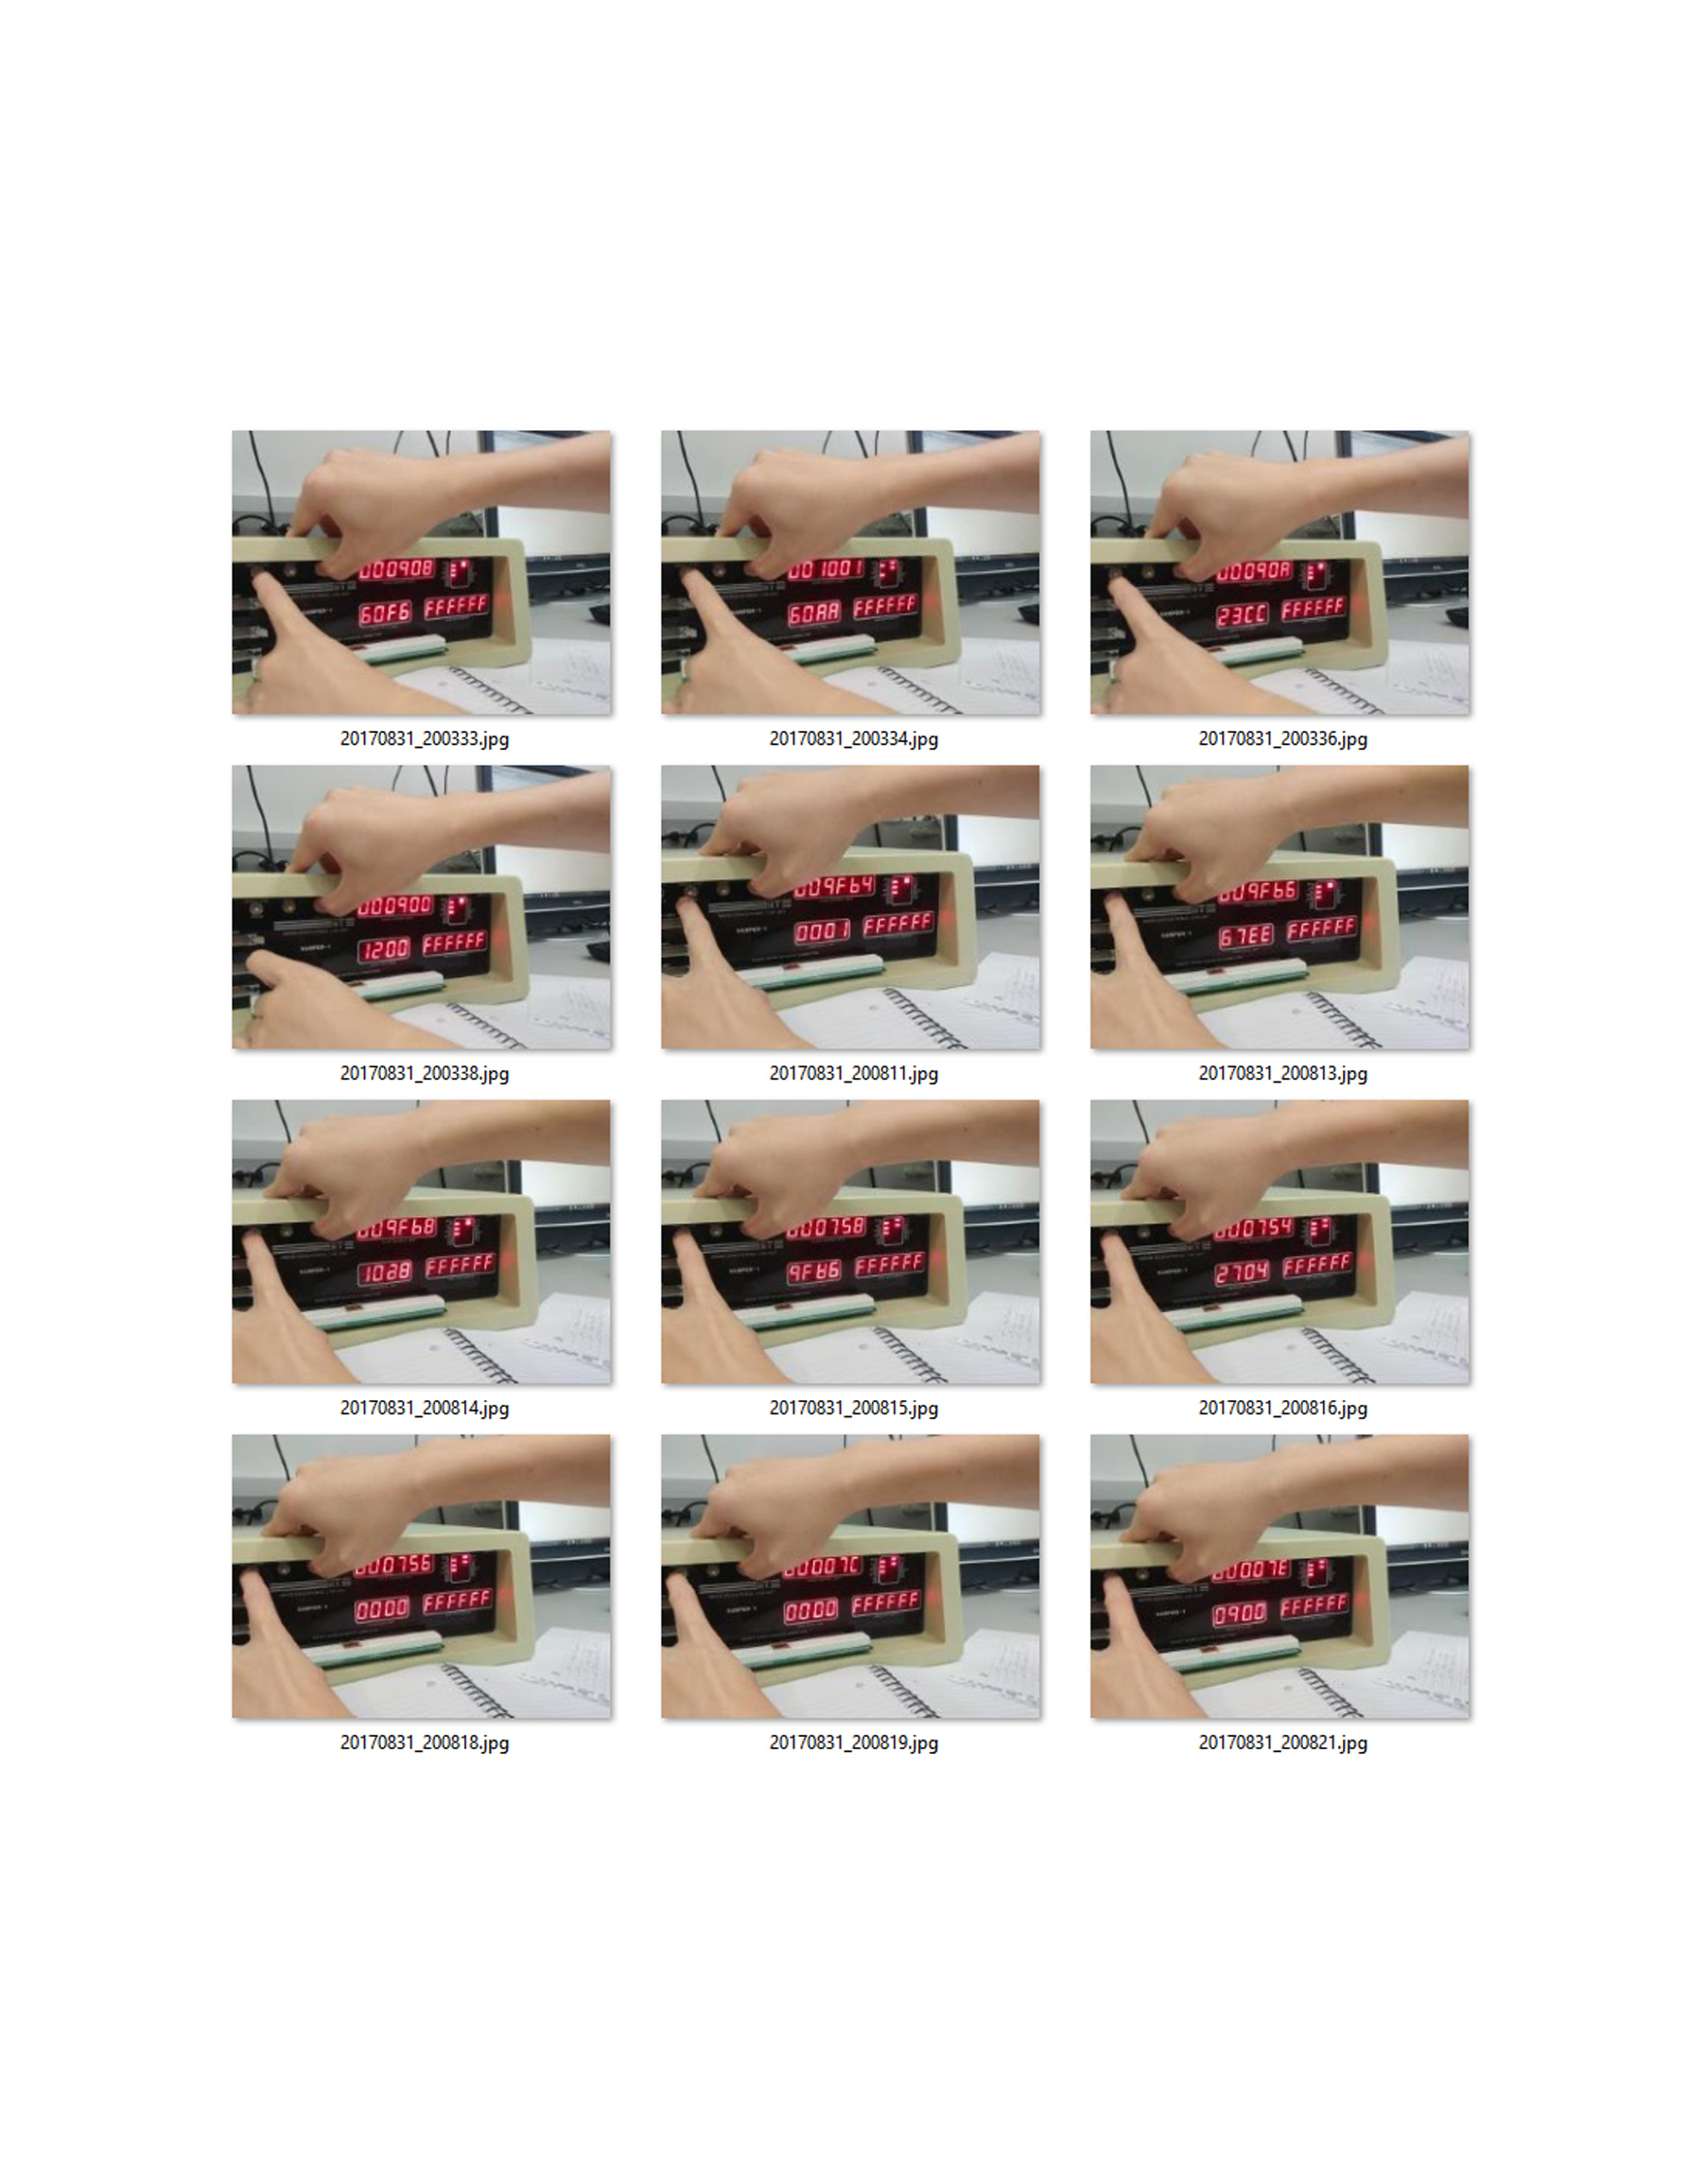
\includegraphics[width=0.9\textwidth]{b3}
					\end{center}\end{figure}
					\begin{figure}[!htb]
					\begin{center}
					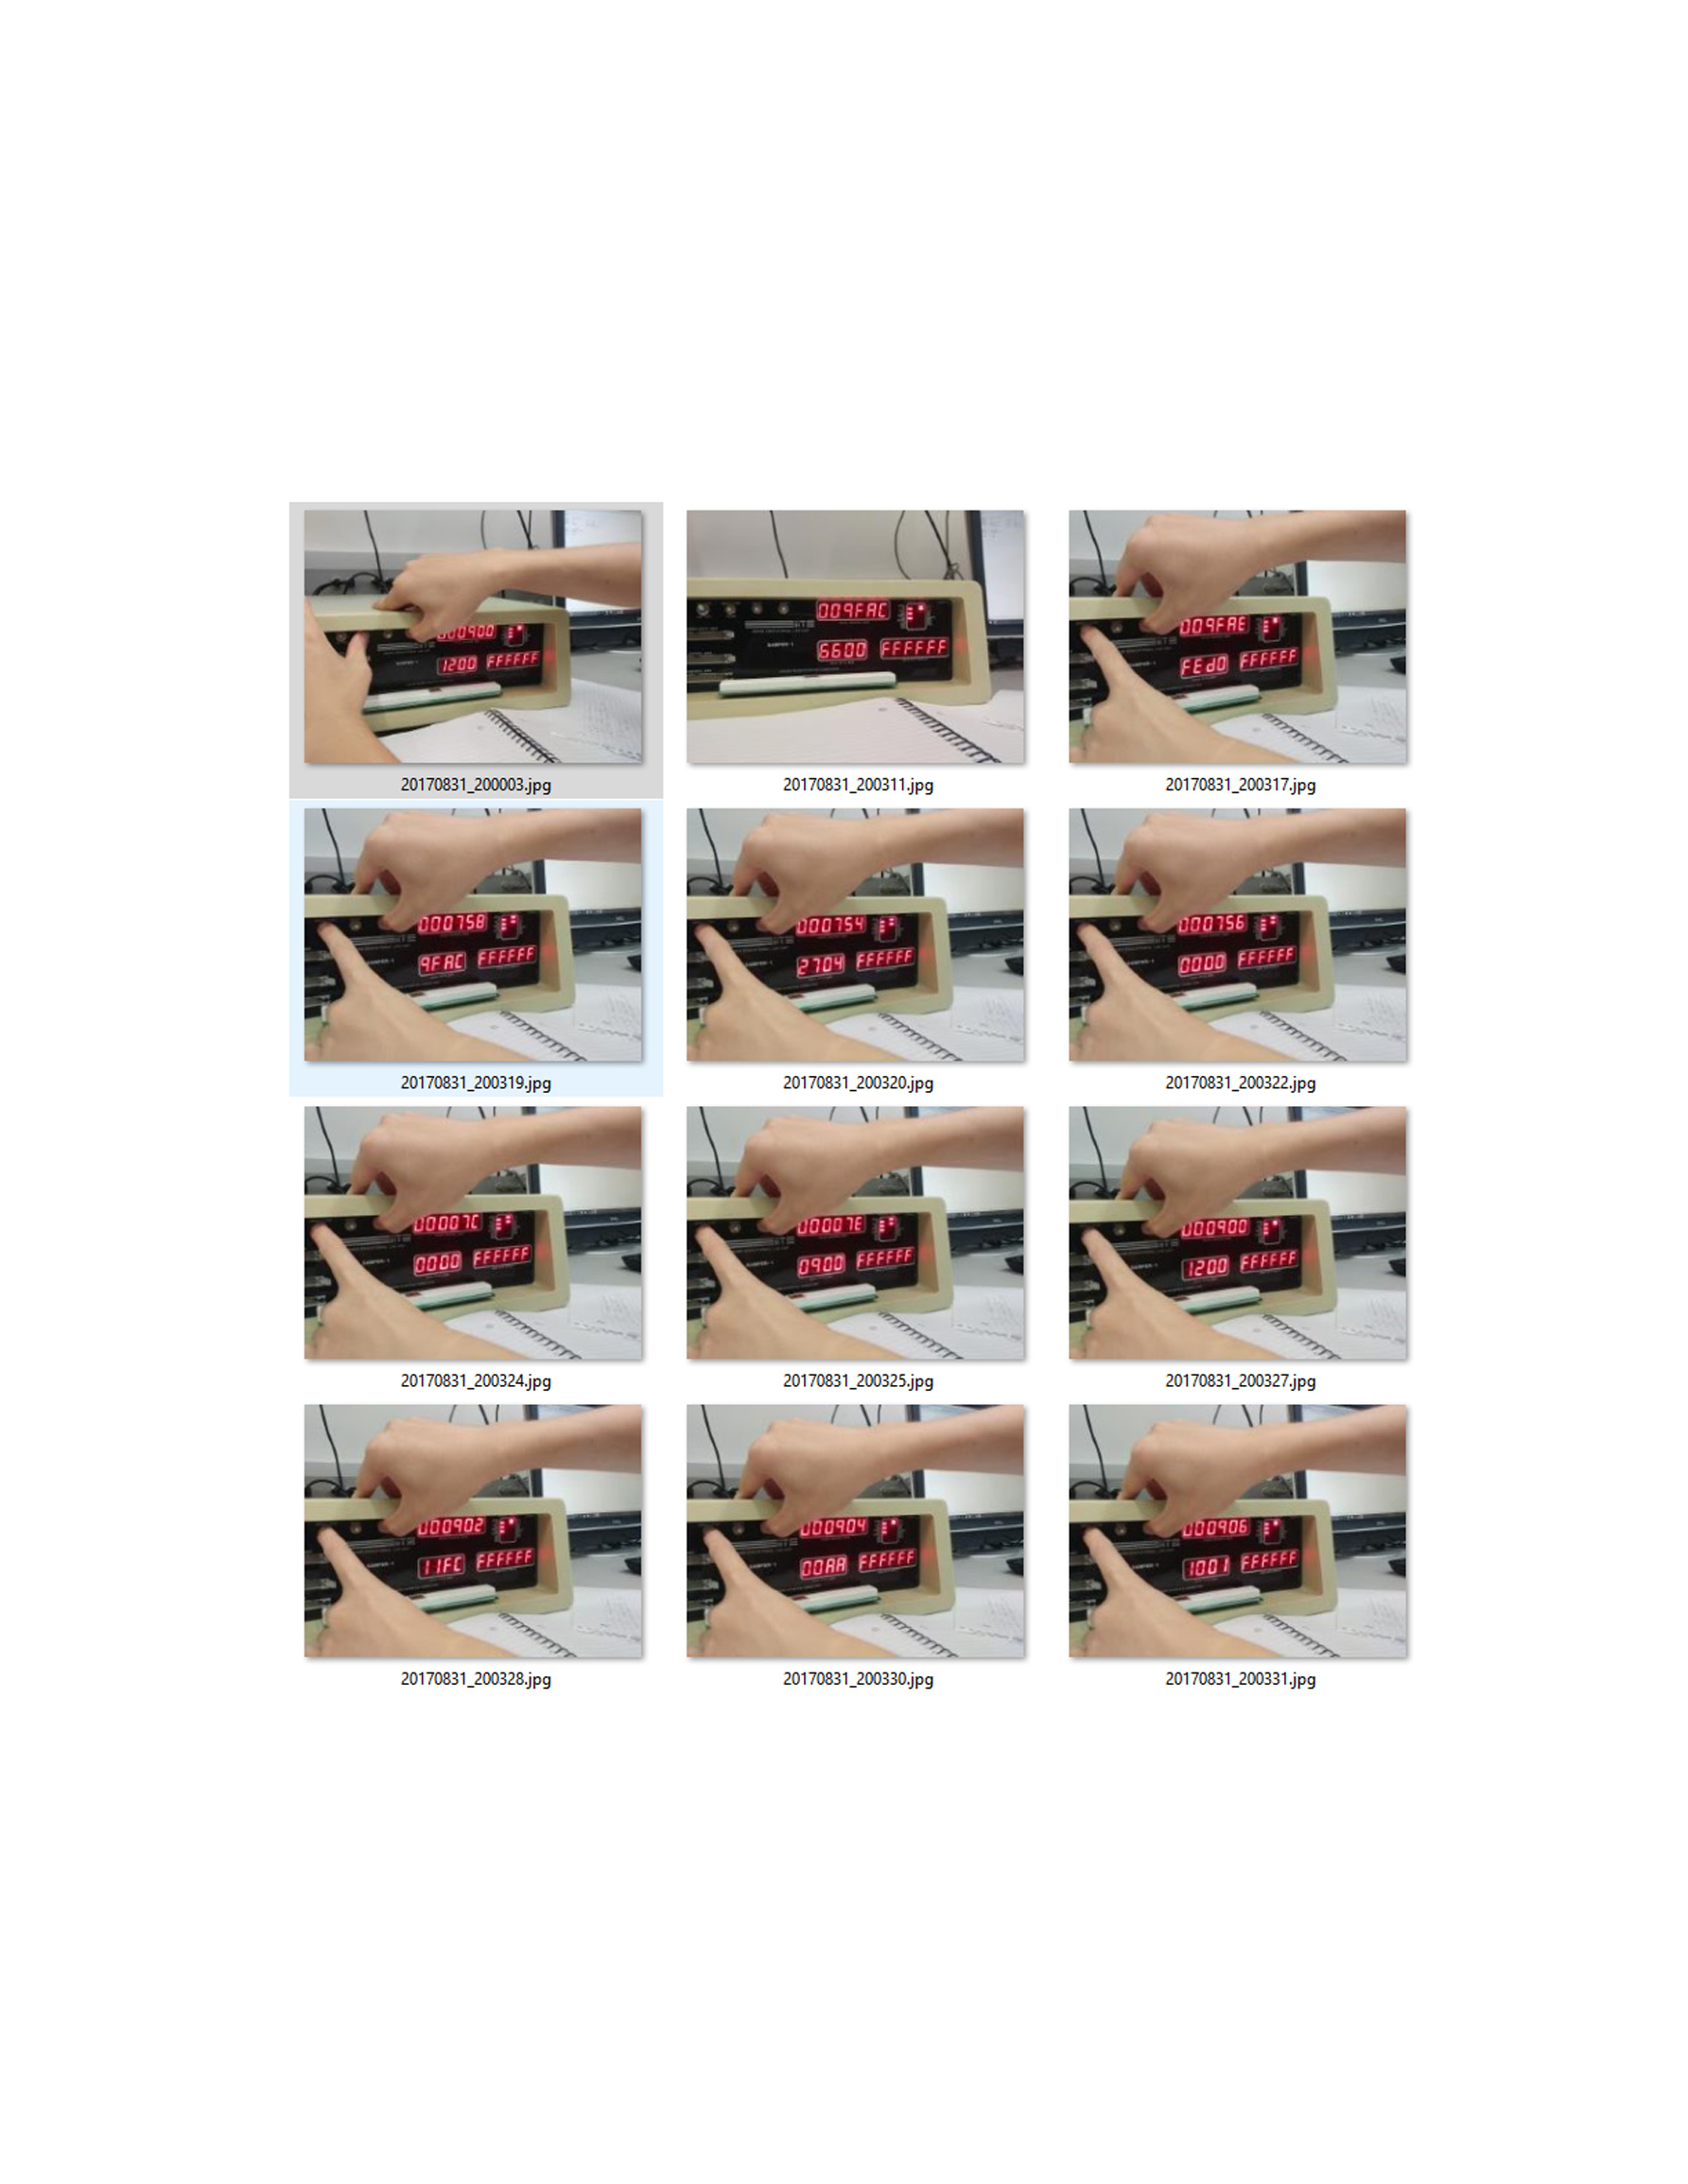
\includegraphics[width=0.9\textwidth]{b2}
					\end{center}\end{figure}
					\begin{figure}[!htb]
					\begin{center}
					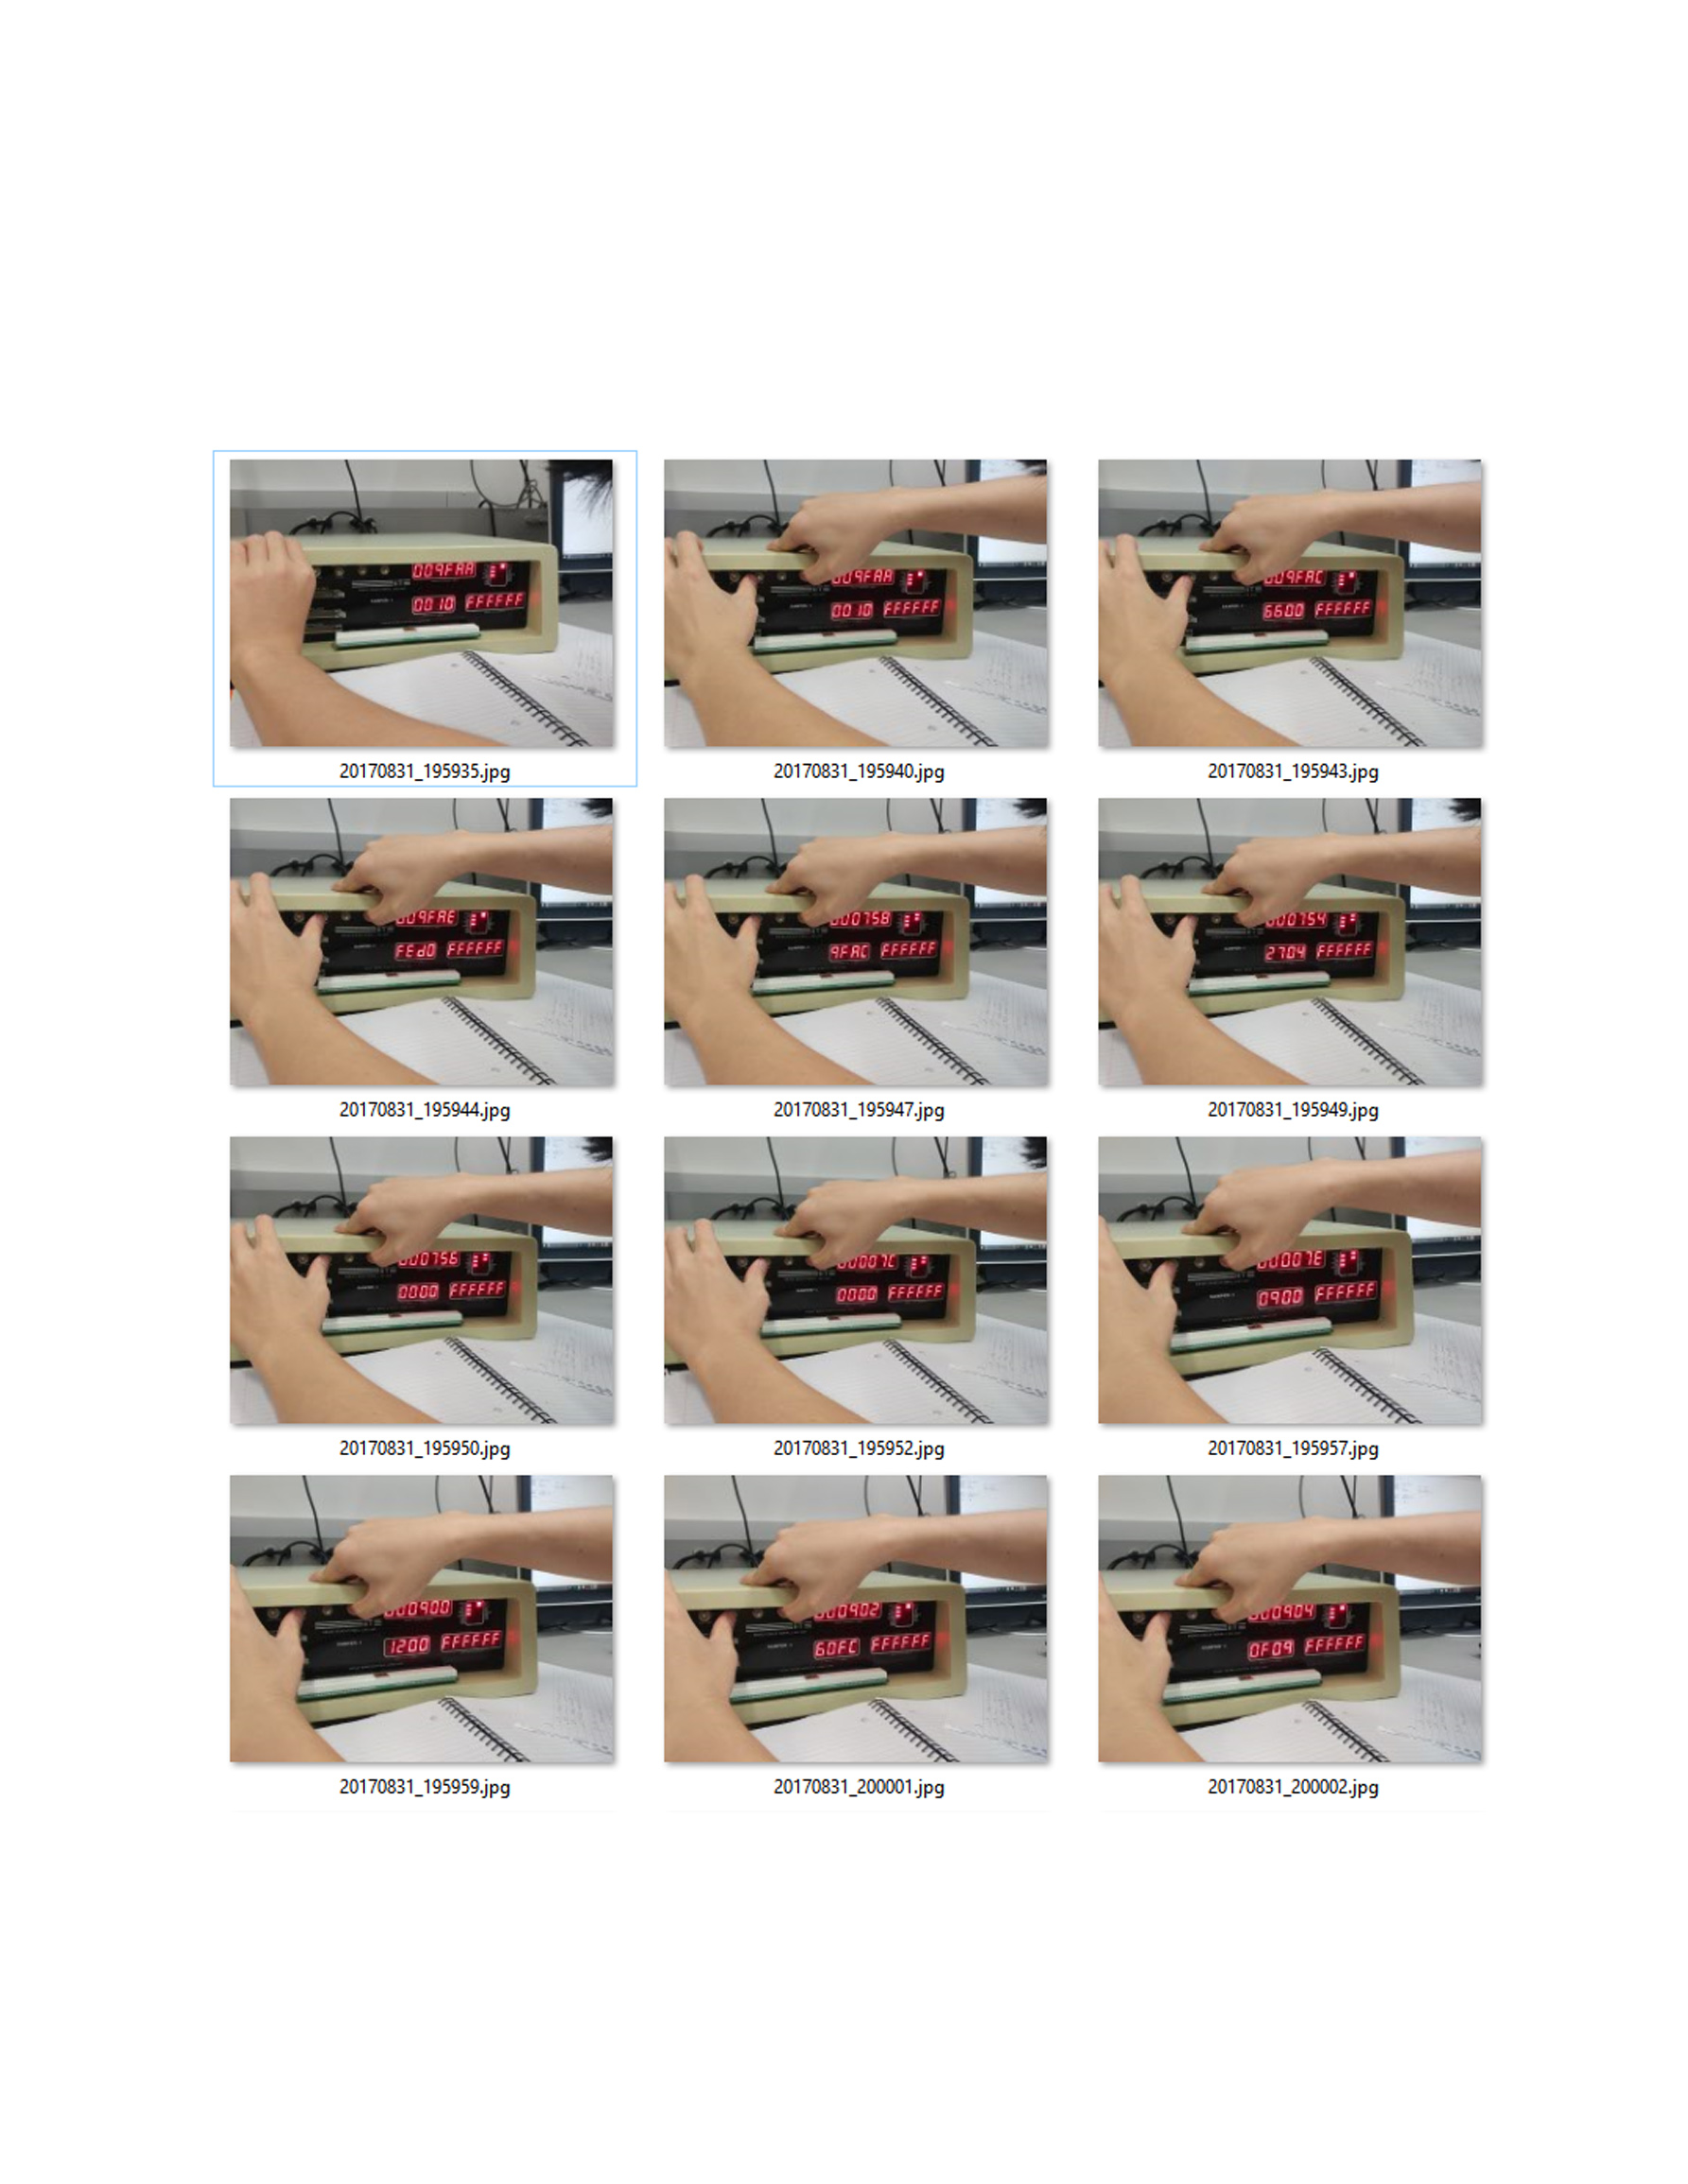
\includegraphics[width=0.9\textwidth]{b1}
					\end{center}\end{figure}
					


\end{document}